\chapter{Conceptual Framework} % Main chapter title

\label{Chapter:ConceptualFramework}

This section of the article opens with an overview of urban agriculture and ends with a conceptual framework for sustainable city.

\section{Overview of urban agriculture}

The Food and Agricultural Organization (2003) defines urban agriculture as any production in the home or plots in an urban area. Central to this definition is the understanding that urban agriculture assumes the nature of farming and gardening in rural areas (Opitz, Berges, Piorr, & Krikser, 2016). Whether to consider peri-urban agriculture as part of urban agriculture or not is a subject that remains unresolved in the conventional literature. While some scholars and organisations limit their description of urban agriculture to only gardens and farms within the inner city (Cohen, Reynolds, & Sanghvi, 2012; Howe, 2002; Kaufman & Bailkey, 2000), others describe it to include agricultural activities in the peri-urban areas (Mok et al., 2014; Pearson, Pearson, & Pearson, 2010; Van der Schans & Wiskerke, 2012). Thebo, Drechsel, and Lambin (2014) make a clear distinction between urban agriculture and peri-urban agriculture based on geographical location. The authors indicate that peri-urban agricultural activities take places within a buffer of 10 to 20 km of the urban geographic boundary. Based on this distinction, the present study focuses on only agricultural activities that take place within an urban geographical boundary or is within 10 km range from a city's core. The work of Ayambire et al. (2019) gives a detailed distinction between urban and peri-urban agriculture.

The purpose of urban agriculture differs between cities in the global south and those in the global north. In the latter, people farm typically for recreational or aesthetic reasons although farming for household food supply becomes pervasive during economic meltdowns (McClintock, 2010). In the former, farming is mainly to satisfy household food needs and for other commercial reasons (Amponsah, Vigre, Braimah, Schou, & Abaidoo, 2016; McClintock, 2010; Tornaghi, 2015). Typically, households in the cities in the global south farm on undeveloped lands, marginal lands and community plots mainly for food for household consumption whereas empty spaces of post-industrial landscapes are being used for agricultural purposes. Rooftops, balconies and more recently vacant lots, road medians, and parks are used for agricultural purposes in the cities in the global north (McClintock, 2010). In this context, urban agriculture is used in the present study to typify crop farming done through community gardens, allotments, backyard gardens and rooftop gardens.

\section{Conceptualising a sustainable city}

The concept of sustainable cities has its roots in the United Nations World Commission on Environment and Development's (UNWCED) idea of sustainable development. The UNWCED summarised sustainable development as meeting the needs of the present generation without compromising the ability of future generations to meet their own needs. The concept has been a standard to strive for in many areas of human activity (Filion, 2017). It is a normative concept that determines theway humans should act towards nature, as well as the way they should be responsible towards one another and future generations (Baumgärtner & Quaas, 2010; Yigitcanlar & Dizdaroglu, 2015). However, Lew, Ng, and Ni (2016) suggest that numerous definitions of sustainability and sustainable development are sometimes sloppy, vague and narrow. This is partly due to the varied understanding of sustainable development and the numerous semantics in the institutional, ideological and academic definitions of sustainability (Mebratu, 1998). For instance, environmental economists believe in economic reductionism by undervaluing ecological goods while social ecologist is reductionist-holistic by focusing on the domination of people and nature. These believes translate into their conception of sustainability and sustainable development. Mebratu (1998), therefore, concludes from the varied conceptions particularly on the cosmic perceptions about the separate existence of nature, economy and society, are problematic for sustainability research. Again, the conceptual understanding and perception of the environment (which comprises living and non-living things) and ecology (which refers to the relationship between living organisms and their environment) as synonymous has affected and continues to affect the conceptual understandings of sustainable development. These can undermine the understanding of a sustainable city since they are intertwined. For clarity, this study's focus on sustainable development considers its tripartite dimension (economic, social and environmental).

In recent times, the sustainable city concept has assumed prominence. This is evident in the Sustainable Development Goal [SDG] 11, which is “to make cities and human settlements inclusive, safe, resilient and sustainable”. The concept's growing prominence is fuelled by rapid urbanisation of the world and the associated effects on environmental quality. The implication is that sustainability should be a crucial objective every development endeavour should strive to achieve (UNHabitat, 2013). In this regard, the primary goal of urban development should be to make cities and their ecosystems healthy and sustainable (Hiremath, Balachandra, Kumar, Bansode, & Murali, 2013; Jovanovic, 2008; Smith, 2015; Thornton, 2011). However, the discourse on urban development and urban sustainability has resulted in a plethora of studies equating the sustainable city concept to the new vision of a compact city. This seems to be a conceptual contention like the definition of sustainable development.

The main idea behind the compact city concept is to have a city that is energy-efficient and less polluting because of the proximity of houses to the market centres, shops and work places (Neuman, 2005). The focus is on compactness, which will result in less travel, efficient use of public transportation and ultimately reduce emissions (Abdullahi, Pradhan, Mansor, & Shariff, 2015; Chang, 2016). Typically, compact cities have less space for green-infrastructure due to the inherent physical and institutional obstacles that limit the quantity and quality of amenity vegetation (Jim, 2004). Studies have also shown that compactness can have adverse effects on domestic living space, affordable housing, and increased crime levels (Chhetri, Han, Chandra, & Corcoran, 2013; Lin, Lin, & Yang, 2006). These effects are contrary to the principles of a sustainable city, which emphasise a balance among economic development, environmental protection, and equity in income, employment, shelter, basic services, social infrastructure and transportation (Hiremath et al., 2013). In this regard, we do not use a compact city interchangeably with a sustainable city in the present study.

The confusion between sustainable city and compact city prompted the authors of this study to provide a clear and comprehensive picture  of the meaning of a sustainable city. As stated earlier, the nuanced conception of sustainable development affects the meaning of a sustainable city. This results in the concentration of indicators that reflect a limited number of dimensions (Tanguay, Rajaonson, Lefebvre, & Lanoie, 2010). However, Hellstro (2000), concludes that it would be unfeasible to try to compile all indicators from all available databases. Therefore, scholars tend to specify on some criteria/indicators based on the focus of their studies and their ideological orientations. For instance, Hellstro (2000) proposed a six study-specific criteria for measuring sustainable urban water management. These criteria are: a) health and hygiene, b) cultural contribution, c) spreading of toxic compounds to water and soil, d) use of natural resources, e) cost benefits, and f) functional risk. The criteria are study-specific and not crosscutting. Many other scholars and organisations use a variety of criteria to define sustainable cities (see: Green City Index, Global City Indicators Facility and the Global Compact Cities Circles of Sustainability). The nuances in the sustainable city indicators are attributable to varied conceptual understanding of a sustainable city discussed above (Alberti, 1996; Egger, 2006; Evans & Marvin, 2006; Portney, 2002).

Models and indices are also backed by conceptual views. As such, there is the need to try to complement the strengths and weaknesses of several indicator-sets to derive a more robust and comprehensive model for measuring sustainable city. The use of indicators is also relevant because they provide a much more detailed and quantitative way of measuring the sustainability of a city. Therefore, in this article we review some of the existing models (the Green City Index, Global City Indicators Facility and the Global Compact Cities Circles of Sustainability) to develop a framework that adequately identifies the indicators for a sustainable city. This framework serves as the basis for the discussion of the role of urban agriculture in sustaining cities.

%\begin{figure}[th]
%\centering
%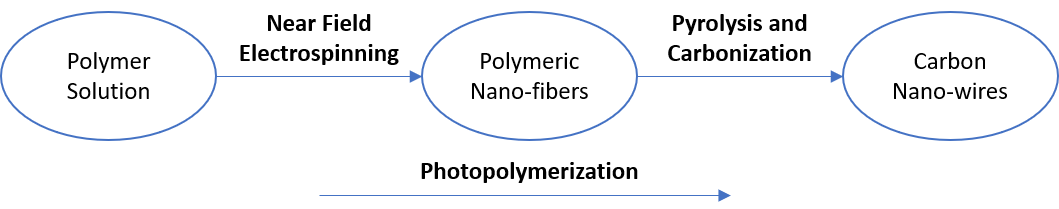
\includegraphics[width=0.95\textwidth]{./Figures/FabricationProcess.png}
%\decoRule
%\caption[Carbon Nano-wires Fabrication Process]{Fabrication process of carbon nano-wires to achieve through the proposed dissertation.}
%\label{fig:fabricationFlowChart}
%\end{figure}

%\begin{equation}
%\left(\tau _t^e-\frac{\tau _n^e \text{dr}}{\text{dz}}\right) 2 \pi  r+\frac{d \left(\pi  r^2
%   \left(\tau _{\text{zz}}-p\right)\right)}{\text{dz}}+\frac{\gamma  \text{dr} 2 \pi  r}{r
%   \text{dz}}+\rho  g \pi  r^2=\frac{d \left(\rho  \pi  r^2 v^2\right)}{\text{dz}}
%\label{eq:linearMomentum}
%\end{equation}